\documentclass[10pt,letterpaper]{article}
\usepackage[margin=0.85in]{geometry}
\usepackage[T1]{fontenc}
\usepackage[utf8]{inputenc}
\usepackage{lmodern,graphicx,booktabs,amsmath,xcolor,hyperref,xurl,caption,fancyhdr}
\hypersetup{colorlinks=true,urlcolor=teal,linkcolor=teal,pdftitle={Paper trail: an explainable recommendation engine and implementation exercise},pdfauthor={James Jean}}
\definecolor{forest}{HTML}{185A43}
\pagestyle{fancy}\fancyhf{}\fancyhead[L]{\small Paper trail / Study 41}\fancyhead[R]{\small Independent research exercise}\fancyfoot[C]{\thepage}
\setlength{\headheight}{14pt}\setlength{\parindent}{0pt}\setlength{\parskip}{6pt}
\captionsetup{font=small,labelfont=bf,hypcap=false}
\begin{document}
{\small\color{forest} RECOMMENDATION SYSTEMS \quad / \quad WORKING PRODUCT + IMPLEMENTATION EXERCISE\par}
\vspace{7pt}
{\LARGE\bfseries Paper trail: related papers,\par with inspectable limits\par}
\vspace{5pt}
James Jean \hfill 29 October 2026

\section*{Decision and verified finding}
Paper trail is a local recommendation engine that suggests related research titles, explains their shared terms, and can abstain. It includes a browser interface, CLI, loopback HTTP API, learner implementation exercise and runnable reference solution. Its practical value is a transparent starting point for reading and an inspectable software exercise; user usefulness and time savings have not been measured.

The selected title-Jaccard rule found at least one deposited citation in its top five for \textbf{12 of 29 evaluable held queries (41.4\%)}. The fixed baseline produced the same outcomes. All 29 held queries were answered: the selected threshold did not improve held citation recovery or reduce held answer coverage. Seventeen answered queries contained no deposited top-five citation; those other suggestions are unjudged, not proven irrelevant.

\textbf{Recommendation.} Use this release to inspect and implement a small recommendation system. Collect independent relevance judgments and a broader frozen corpus before claiming better discovery or deploying recommendations for others. A matching title does not establish that a paper supports a claim.

\begin{center}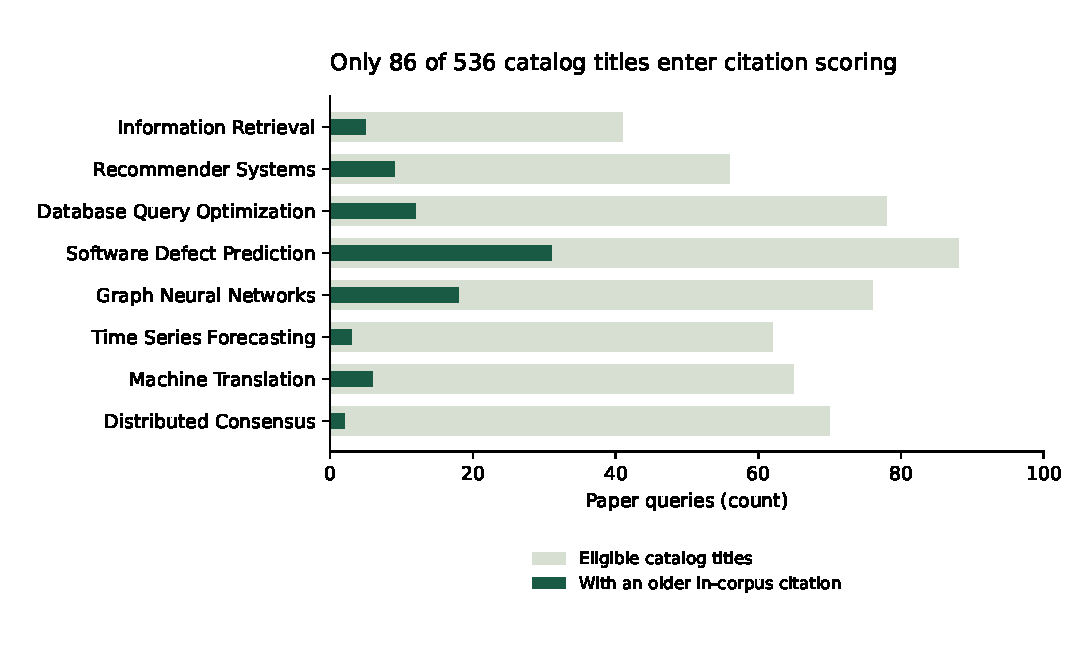
\includegraphics[width=.94\linewidth]{images/corpus_coverage.pdf}\end{center}
\captionof{figure}{A selective evaluation population. Only 86 of 536 catalog titles have an older, in-corpus deposited reference: 57 development and 29 held queries. The other 450 titles remain in the catalog and coverage file. Request strata are acquisition labels, not verified scientific topics.}

\textbf{Scope.} This is a descriptive retrospective citation-proxy experiment with a working teaching prototype, not peer reviewed research, human relevance validation, evidence certification, a novel estimator or a production deployment. Separate formal-publication projects, including Azure optimization, are excluded.

\newpage
\section*{1. Source and evaluation population}
Eight fixed public Crossref requests each requested up to 100 records using a title query, the publication window 2018--2024 and the has-references filter. The protocol was pushed before the corpus was collected. Requests were serial, unauthenticated and rate limited; no paid service, credentials, alternative query expansion or full-text retrieval was used. The capture contained 800 returned records: 536 eligible unique journal/proceedings articles, 264 exclusions under the fixed rules and no duplicate eligible DOI records.

Raw responses and captured source documentation remain private. Public projections contain DOI, cleaned first title, publication year, article type, query-stratum provenance and DOI-only reference identifiers. Abstracts, full papers, expressive reference strings, authors, affiliations, contact details, funding and personal profiles are excluded. Crossref permits metadata reuse while warning that some abstracts have separate copyright [1--3]. Source deposits may be incomplete or wrong.

\begin{center}\small
\begin{tabular}{lrrl}\toprule
Request stratum & Catalog & Evaluable & Partition\\\midrule
Information Retrieval & 41 & 5 & Dev. \\
Recommender Systems & 56 & 9 & Dev. \\
Database Query Optimization & 78 & 12 & Dev. \\
Software Defect Prediction & 88 & 31 & Dev. \\
Graph Neural Networks & 76 & 18 & Held \\
Time Series Forecasting & 62 & 3 & Held \\
Machine Translation & 65 & 6 & Held \\
Distributed Consensus & 70 & 2 & Held \\
\bottomrule\end{tabular}
\end{center}

Each unique DOI is a potential query using only its own title. Candidate titles must have a strictly earlier publication year. Deposited reference DOIs that intersect those candidates form the proxy positives. No-positive queries are excluded from citation-scoring denominators and retained in coverage output; their relevance is unknown. The evaluable fraction is 57/263 in development and 29/273 in held strata, not all catalog users or all scholarly literature.

Unique query DOIs do not cross partitions. Candidate records can be shared across query partitions; this is a held-query-stratum evaluation rather than a fully disjoint topic or catalog test. The current captured metadata and deposited references are retrospective; historical availability and prospective operation are unverified. The strict older-year rule also excludes same-year and pre-2018 uncaptured work.

\section*{2. Transparent, fixed ranking rules}
The engine uses NFKC/casefold normalization, ASCII letter/digit tokens of length at least two and the explicit stop list in the executable protocol. This English-oriented rule has no stemming, translation or semantic synonym model. Jaccard is the shared token-set size divided by the union size. The comparator uses log term frequency and smoothed IDF:
\[
w_{td}=(1+\ln c_{td})\left[1+\ln\frac{N+1}{df_t+1}\right],\qquad
s(q,d)=\frac{w_q^\top w_d}{\|w_q\|_2\|w_d\|_2}.
\]
IDF uses only the query's eligible older candidate titles; unseen query tokens have zero cosine weight. These are established lexical methods [4], implemented with the standard library, not an embedding model or new estimator. Ranker features exclude reference labels and acquisition strata.

\newpage
\section*{3. Selection before held outcome summaries}
Candidates need at least two shared tokens and a positive score. Scores are rounded to 12 decimals, then sorted descending with ascending DOI tie breaking. If the top score falls below the query threshold, the engine abstains. Otherwise it returns up to five positive two-term matches; lower-ranked items need not individually exceed that threshold. Scores are lexical similarities, not probabilities or calibrated confidence.

The fixed grid has two rankers and five thresholds, with no extensions. Development selection maximizes equal-query mean proxy utility: +1 when an answered query has a deposited top-five citation, $-0.25$ when answered without one, and zero when abstaining. The penalty is a hypothetical teaching tradeoff; no human cost was measured. Ties prefer a lower threshold, then Jaccard.

\begin{center}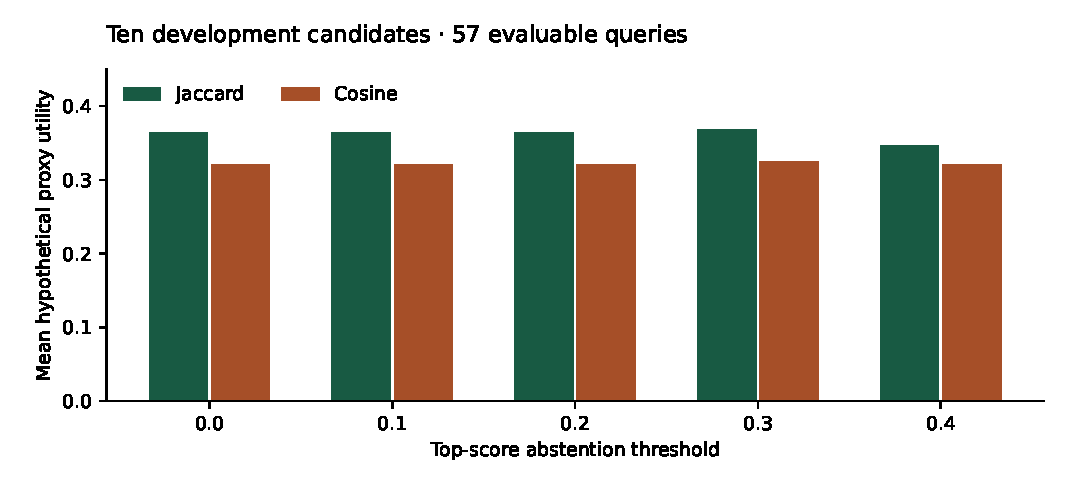
\includegraphics[width=.96\linewidth]{images/development_search.pdf}\end{center}
\captionof{figure}{All ten development candidates. Differences describe this finite 57-query snapshot. The selected Jaccard threshold of 0.3 abstains on one development query, retaining 28 top-five citation hits. No statistical significance, global optimum or user benefit is inferred.}

\begin{center}\small
\begin{tabular}{lrrrr}\toprule
Ranker & Threshold & Answered /57 & Hits /57 & Mean utility\\\midrule
Jaccard & 0.0 & 57 & 28 & 0.364035 \\
Jaccard & 0.1 & 57 & 28 & 0.364035 \\
Jaccard & 0.2 & 57 & 28 & 0.364035 \\
Jaccard & 0.3 & 56 & 28 & 0.368421 \\
Jaccard & 0.4 & 46 & 25 & 0.346491 \\
Cosine & 0.0 & 57 & 26 & 0.320175 \\
Cosine & 0.1 & 57 & 26 & 0.320175 \\
Cosine & 0.2 & 57 & 26 & 0.320175 \\
Cosine & 0.3 & 56 & 26 & 0.324561 \\
Cosine & 0.4 & 52 & 25 & 0.320175 \\
\bottomrule\end{tabular}
\end{center}

The selected rule has exact development utility $7/19$. Thirty-four source, protocol, code, exercise, test, UI and development-result dependencies were hashed and committed at revision \texttt{7220b9e} before the separate held command. Full source reference metadata was visible during development; this is a chronology of frozen selection, not a claim of analyst blinding. A pre-held CSV line-ending correction preserved semantics, source, candidate scores and the selection. The earlier bytes are retained privately.

\newpage
\section*{4. Held outcomes and failures}
The frozen rule and baseline both answer 29 queries, with 12 deposited-citation hits. Their identical metrics do not establish general equivalence. Hit@5 is the fraction of evaluable queries with at least one deposited top-five reference. Recall averages the fraction of each query's in-corpus positives retrieved; reciprocal rank is zero when no positive appears. Missing deposited edges are not independent negative relevance labels.

\begin{center}\small
\begin{tabular}{lrr}\toprule
Metric & Selected: Jaccard 0.3 & Baseline: Jaccard 0\\\midrule
Answered queries & 29 & 29 \\
Queries with a top-five citation & 12 & 12 \\
Hit@5, all evaluable queries & 0.413793 & 0.413793 \\
Macro deposited-reference recall@5 & 0.396552 & 0.396552 \\
Mean reciprocal rank@5 & 0.300000 & 0.300000 \\
Hypothetical mean proxy utility & 0.267241 & 0.267241 \\
\bottomrule\end{tabular}
\end{center}

\begin{center}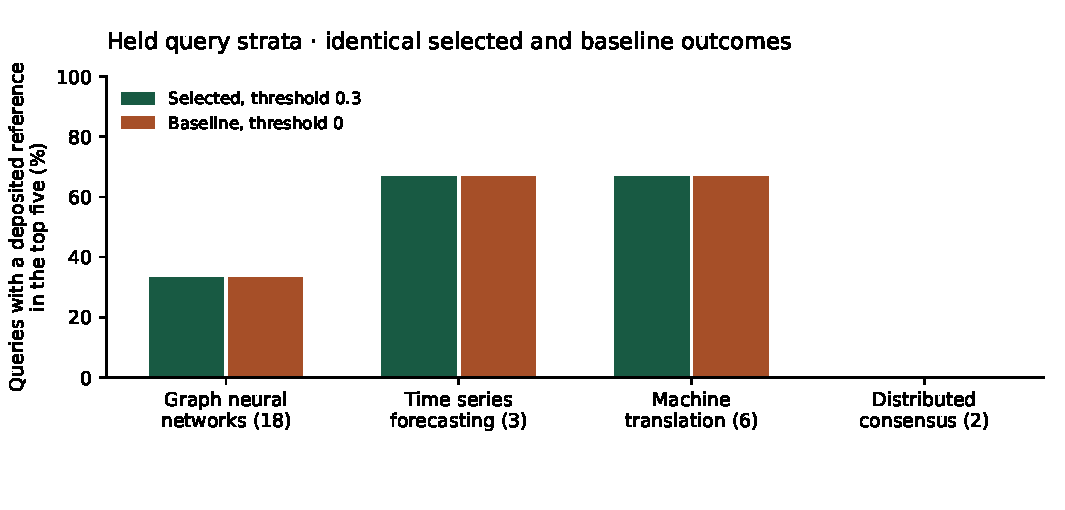
\includegraphics[width=.96\linewidth]{images/held_strata.pdf}\end{center}
\captionof{figure}{All four held acquisition strata, with query counts in parentheses. Small strata are descriptive. Distributed consensus has zero hits in two queries; no subgroup was removed or used to retune the model. Both rules have the same bar heights.}

\begin{center}\small
\begin{tabular}{lrrr}\toprule
Held stratum & Queries & Top-five hits & Mean utility\\\midrule
Graph Neural Networks & 18 & 6 & 0.166667 \\
Time Series Forecasting & 3 & 2 & 0.583333 \\
Machine Translation & 6 & 4 & 0.583333 \\
Distributed Consensus & 2 & 0 & -0.250000 \\
\bottomrule\end{tabular}
\end{center}

The engine abstained on all eight prespecified synthetic unrelated queries. They are authored negative controls, not independent human relevance judgments or general out-of-domain safety evidence. The 17 held no-hit queries remain exported beside the successful queries; their other suggestions have not been adjudicated. No confidence interval or significance claim is made for this selected finite snapshot.

\newpage
\section*{5. Working product and learner implementation}
The browser interface accepts a public title or known catalog DOI and displays up to five titles, DOI links, years, lexical scores and matching tokens. A known DOI resolves locally to its title, excludes itself and limits candidates to earlier years. A free-text search uses the full catalog unless the optional before-year field is set. The held research evaluation always uses the older-year rule; arbitrary live free-text behavior has not been evaluated with human labels.

The same reference ranker serves the CLI and JSON API. The HTTP service binds only to loopback, checks host and origin boundaries, accepts a bounded JSON body, exposes only fixed static paths, and does not log or forward queries. There is no paid API, remote inference, personal profile, telemetry, stored query history or private manuscript input. External DOI links open only when the reader chooses to follow one. These implementation checks do not establish universal application security.

\textbf{Run locally.} From the checkout, run \texttt{python -m recommender.server} and open \url{http://127.0.0.1:18341/}. The runtime engine and service use Python's standard library. The CLI is \texttt{python -m recommender "graph neural networks"}. Pinned dependencies support collection, independent numerical checks, figures and PDF validation.

\textbf{Implementation exercise.} Learners implement the pure Jaccard ranker in \texttt{exercises/ranker.py}: normalization, set arithmetic, two-term eligibility, deterministic ties, explanatory terms and nonmutation of inputs. The initial stub deliberately exits the grader with status 2 and INCOMPLETE. It is not claimed to be a completed learner answer. The runnable reference in \texttt{exercises/reference.py} imports the production pure implementation, avoiding a second divergent solution. Ten hand contract assertions test the reference; the broader product suite has 17 tests covering ranking, labels, thresholds, dates and API boundaries.

\textbf{Interface inspection.} The current interface was inspected in Chrome at 1718-pixel desktop width and 390 by 844 phone size. Both showed no horizontal overflow; all five phone result cards remained within the content width. The known-DOI example excluded its seed and used 442 older candidates. Labels, live status text, the abstention message and a visible three-pixel keyboard focus outline were checked. No warning/error entries were returned for the inspected app tab. This finite check does not establish accessibility conformance, screen-reader usability or general browser compatibility.

\section*{6. Independent evidence and reproduction}
Source reconciliation compared 16,228 values/checks with the private captured responses. Independent NumPy ranking, SQL older-year/citation joins and exact rational metrics passed 26,812 development and 4,316 held checks. These checks do not import the production ranking or scoring helpers. Independent score tolerance is $2\times10^{-12}$ absolute; counts, ranks, fractions and selection utility are exact.

An isolated offline replay matched 32,518 exact CSV fields, 10,319 explanatory contribution values within the same declared tolerance and four JSON documents. It also reran all 17 tests and the reference exercise contract, verifying the learner stub's expected incomplete status. The three original figures have 34 independently matched bar values, 272 SVG coordinate checks and nine file hashes. These are finite checks, not universal correctness or external scientific validation.

\newpage
\section*{7. Limits and next evidence}
The corpus is a fixed, search-ranked slice of 2018--2024 metadata, not a representative literature sample. Only 86 of 536 eligible titles enter citation scoring. Source exclusions, all coverage denominators, every attempted model/threshold and all query-level failures remain public. Current deposited metadata can include errors, incomplete citation lists and later corrections. No original historical release vintage was established.

Title similarity misses synonyms, nuanced methods and contexts of citation. Different works can have the same title; DOI identity and lexicographic ties are explicit, but there is no semantic work-family deduplication. The query-stratum split does not guarantee independent topics or related-work families. Citation recovery can reward well-indexed, older or frequently cited work and does not determine whether a citation supports, criticizes or merely mentions another paper. There are no independent human relevance labels, claim-support assessments, quality ratings or retraction screening in this release.

The selected threshold avoided one development answer and changed no held answer. Eight successful synthetic abstentions cannot establish broad rejection performance. No probabilities, calibrated uncertainty, statistically significant gains, human time savings, realized impact, deployment or production-user counts are claimed. The implementation exercise demonstrates finite engineering behavior; passing its grader is not a research-validity certificate.

\textbf{Next step.} For a decision-specific extension, define the reader task and obtain independent relevance judgments before model selection. Fix a broader, eligible corpus and held queries with work-family and topic separation appropriate to that task. Compare the simple baseline with any proposed semantic model under an explicit compute/rights budget. Retain rejected matches and human disagreement. A support-verification product would additionally require access to eligible source content and passage-level evidence checks; this title recommender does not provide them.

\section*{Reproduce and inspect}
Install \texttt{requirements.txt}, run \texttt{python src/reproduce.py}, then the independent source, figure, manuscript and canonical-Git checks listed in the workflow. The offline replay uses the published minimal snapshot, not live search results. Full-source reconciliation requires the separately retained private originals; public hash/schema checks cannot independently prove those originals. Repeating the captured requests can produce changed current results and is not a historical snapshot reproduction.

The repository retains the executable protocol, data rights, frozen dependency hashes, complete selection table, per-query/ranked exports, coverage exclusions, checks, screenshots, implementation exercise, source code and this manuscript. Public release requires exact-head Linux CI, identical tested/merged trees and a verified remote annotated tag; this document's local checks alone are not a claim those later remote gates have passed. Formal-publication projects remain private.

\section*{References}
{\small
[1] Crossref. REST API. \url{https://www.crossref.org/documentation/retrieve-metadata/rest-api/}. Accessed 29 October 2026.\par
[2] Crossref. Access and authentication. \url{https://www.crossref.org/documentation/retrieve-metadata/rest-api/access-and-authentication/}. Accessed 29 October 2026.\par
[3] Crossref. Metadata retrieval. \url{https://www.crossref.org/documentation/retrieve-metadata/}. Accessed 29 October 2026.\par
[4] Scikit-learn. Feature extraction: TF--IDF term weighting. \url{https://scikit-learn.org/stable/modules/feature_extraction.html}. Accessed 29 October 2026. Method documentation only; no scikit-learn model was used.}
\end{document}
